\chapter {Scilab Based Circuit Simulation}

Electronic circuit simulation uses mathematical models to replicate the behavior of an electronic circuit. Unfortunately, no simulator gives the system of equations it solves, in order to get the solution. In Oscad there is an option to simulate the circuit using SMCSim(Scilab Based Mini Circuit Simulator)An important feature of SMCSim is that it gives the system of equations for the circuit under test. The SMCSim works in three modes: normal, symbolic and numerical mode. In normal mode, SMCSim solves the circuit and gives the final output. In symbolic mode, it gives symbolic equations along with the result. In numerical mode, it gives symbolic equations, intermediate numerical values of the components and entries in system matrices, and the final output. Here, we present the working and implementation of SMCsim with an example. 

Consider Half-Wave Rectifier with Filter shown in Figure \ref{br}.The circuit is drawn using Eeschema integrated with Oscad and spice compatible netlist is generated using Oscad circuit simulation tools. The generated netlist is given below. Note that this netlist is generated for SMCSim which has a simple model implementation for a diode. Thus, users need to specify only Is and Vt values.\\

------------------------------------------------\\ 
Half-Wave Rectifier \\
V1 1 0 sine (5 50) \\
D1 1 2 mymodel (1e-8 0.026)\\ 
R1 2 0 10000 \\
C1 2 0 10e-3 \\
.tran 0 100 0.5\\ 
.plot v(1) v(2) \\
.end \\
------------------------------------------------\\

\begin{figure}[h]%h stands for 'here'. If h is removed then the fig will go to the bottom or to the next page.
\begin{center}
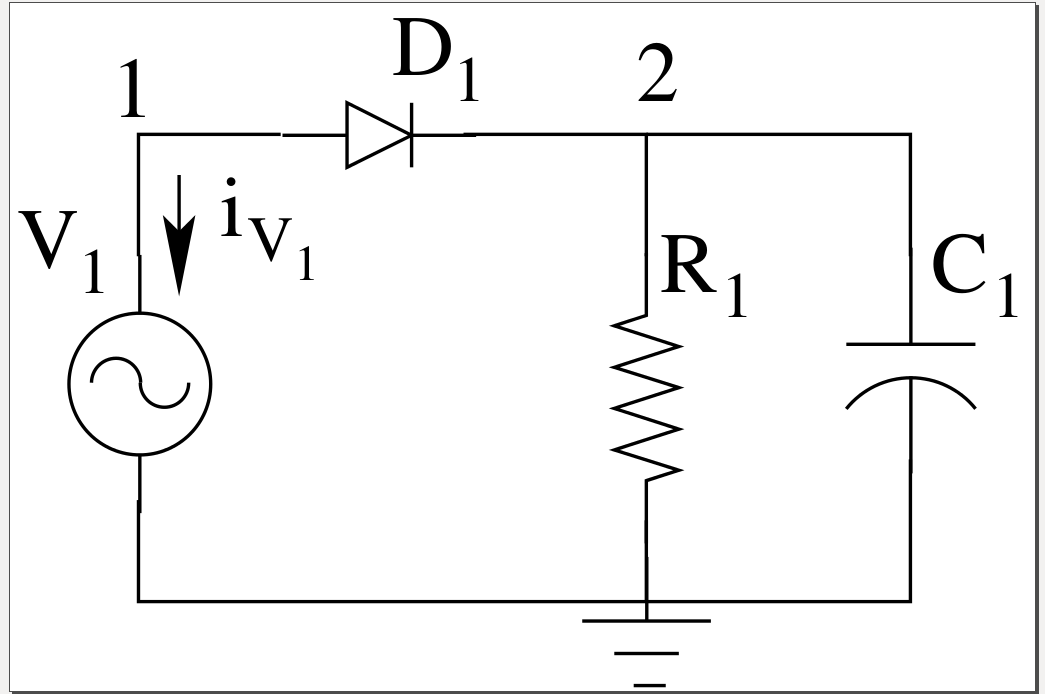
\includegraphics[width=1\linewidth]{figures/bridge-rectifier-circuit.png}%If the fig is appearing too big/small, change the scaling factor 0.2
\caption{Bridge rectifier circuit}
\label{br}
\end{center}
\end{figure}

SMCSim firstly read the netlist and create a graph corresponding to it using Scilab based graph library “metanet”. Then circuit is translated into circuit equations using a circuit equations formulation method. All the methods of formulating circuit equations use Kirchhoff’s current and voltage equations (KCE and KVE), and device characteristics constraints but differ in the manner in which these constraints are imposed [11]. We have used Modified Nodal Analysis (MNA) [12] as it is applicable to all kinds of electrical circuits. Using MNA m ethod and graph operations, we have efficiently built the circuit equations. The system of Equations representing the electrical circuit shown in Figure 4 is given below. SMCSim has capability to display these equations.\\

-------------------------------------------------\\
iV1 + D1f (v1 , v2 ) = 0 \\
(R1 )v2 + (C1 ) (dv2/dt)+ - D1(v1, v2)=0\\

v1=V1\\

 
+ −D1f (v1 , v2 ) = 0\\ 
dt \\
v1 = V1\\ 

Dnf (va , vb ) = Isn (1 − e(va −vb )/vtn )\\ 
where Isn =reverse saturation current and vtn =threshold voltage of diode n\\ 
------------------------------------------------\\
Now, we explain how SMCSim performs Operating point (DC) analysis and Transient analysis.
(DCI) 

\section {Operating Point (DC) Analysis}: 
A circuit can reach an equilibrium point only when stimulus is constant. So, first step of operating point analysis is to configure the independent sources such that they are constant[13]. Since all waveforms are constant-valued at equilibrium points, dv/dt = 0 and di/dt = 0 and so capacitors act as open circuits and inductors act as short circuits. Thus, for operating point analysis, SMCSim removes the time-dependent components properly. The equations that describe the resulting system are nonlinear and algebraic and solution gives equilibrium point. The equations for the circuit are given below: \\
-------------------------------------------------------\\

iV1 + D1f (v1 , v2 ) = 0                                    (4) \\
(R1 )v2 + −D1f (v1 , v2 ) = 0                               (5) \\
v1 = V1                                                    (6) \\
Dnf (va , vb ) = Isn (1 − e(va −vb )/vtn ) \\

where Isn =reverse saturation current and vtn =threshold voltage of diode n\\ 
---------------------------------------------------------\\

Generally for nonlinear devices, a linear model is con- structed that is valid only locally around a point [14]. We have used Newton-Raphson method to construct a linear model for a nonlinear devices. In the example, diode D1 is a nonlinear device. SMCSim constructs the linear model for diode D1 as shown in the Figure \ref{lin}. Note that the value of resistor and current source changes at every iteration and SMCSim allows user to observe the value. This is very useful for debugging the circuit when the simulation is not converging. The system of equations representing the linearized electrical circuit is given below:\\ 
------------------------------------------------------------\\
(RD1 )v1 + (−RD1 )v2 + iV1 = −iD1                        (7)\\
(RD1 )v1 + (RD1 + R1 )v2 = iD1                            (8)\\
v1 = V1                                                  (9) \\
-------------------------------------------------------------\\

\begin{figure}[h]%h stands for 'here'. If h is removed then the fig will go to the bottom or to the next page.
\begin{center}
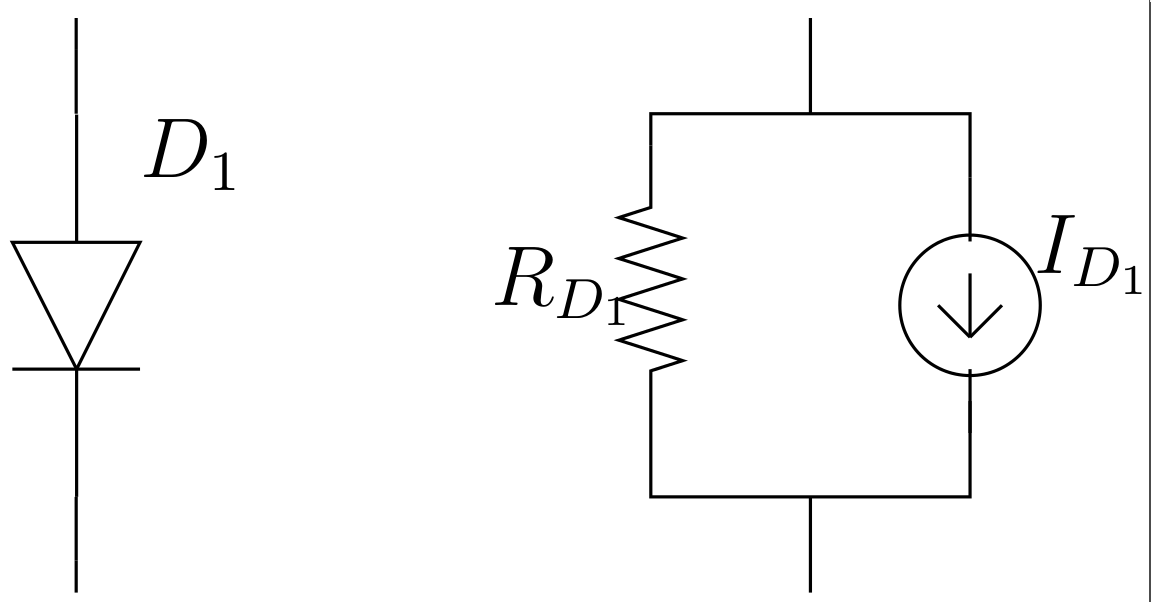
\includegraphics[width=1\linewidth]{figures/diode-linearization.png}%If the fig is appearing too big/small, change the scaling factor 0.2
\caption{Diode model linearisation}
\label{lin}
\end{center}
\end{figure}




\section {Transient Analysis:}

In transient analysis, time dependent components are discretized, i.e., for dynamic devices, a static model is constructed, using a numerical integration method, that is valid for a particular time point. The circuit contains capacitor C1 , as a dynamic device. To solve the circuit, SMCSim constructs a static model for the capacitor C1 using Backward Euler method and performs operating point analysis for a time instant t. The operating point solution gives the solution at time instant t. Note that for each time instant, the values of the static model and the voltage source change. 

Now let us take an example of Bridge Rectifier circuit shown in the schematic given in Figure \ref{bschem} and see how to do “Scilab based circuit simulation”


\begin{figure}[h]%h stands for 'here'. If h is removed then the fig will go to the bottom or to the next page.
\begin{center}
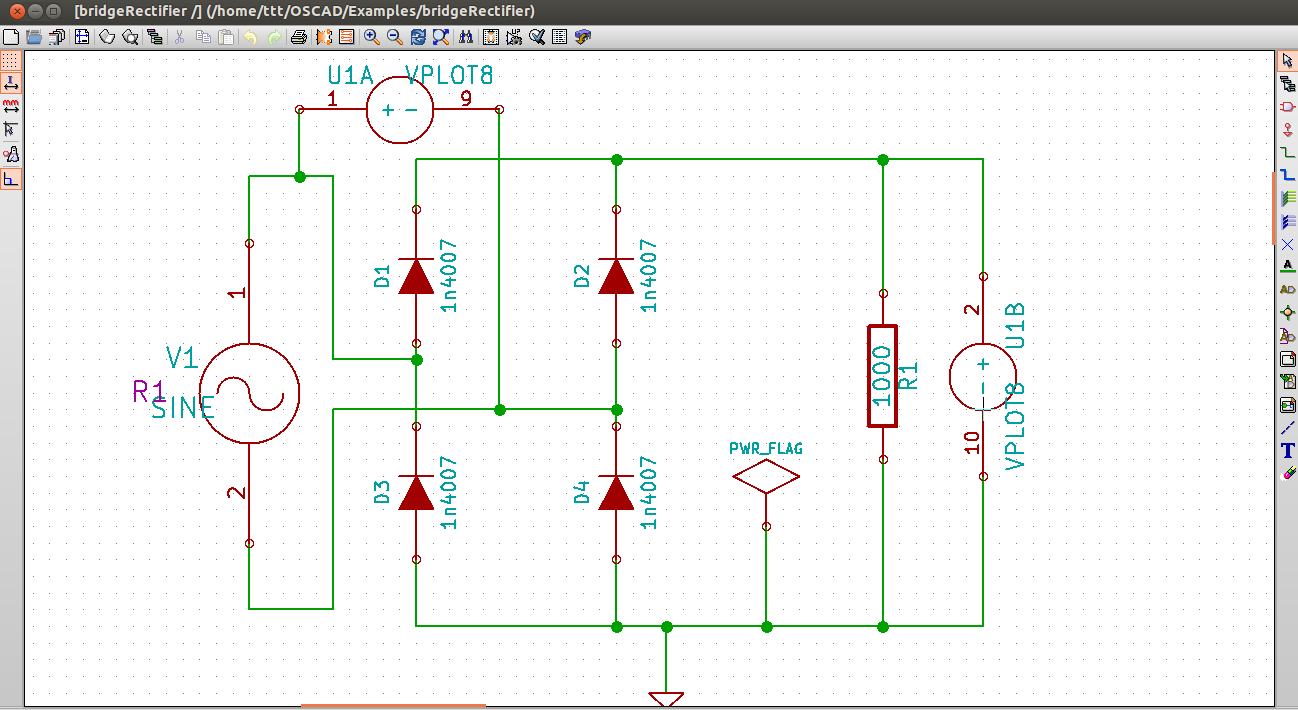
\includegraphics[width=1\linewidth]{figures/SMCSim-B-Rectifier.png}%If the fig is appearing too big/small, change the scaling factor 0.2
\caption{Bridge rectifier circuit schematic}
\label{bschem}
\end{center}
\end{figure}

To go for Scilab based simulation you will have to follow all the steps of simulations explained in the chapter “?” on simulations and finally click on the button of “SMCSim” on the Oscad “Tool Bar” as shown in Figure \ref{smc}.

\begin{figure}[h]%h stands for 'here'. If h is removed then the fig will go to the bottom or to the next page.
\begin{center}
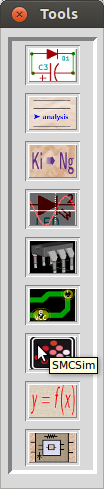
\includegraphics[width=1\linewidth]{figures/select-SMCSim.png}%If the fig is appearing too big/small, change the scaling factor 0.2
\caption{Select SMCSim from Oscad toolbar}
\label{smc}
\end{center}
\end{figure}

And then you will see the the output of the Scilab based simulations as shown in Figure \ref{sci}.

\begin{figure}[h]%h stands for 'here'. If h is removed then the fig will go to the bottom or to the next page.
\begin{center}
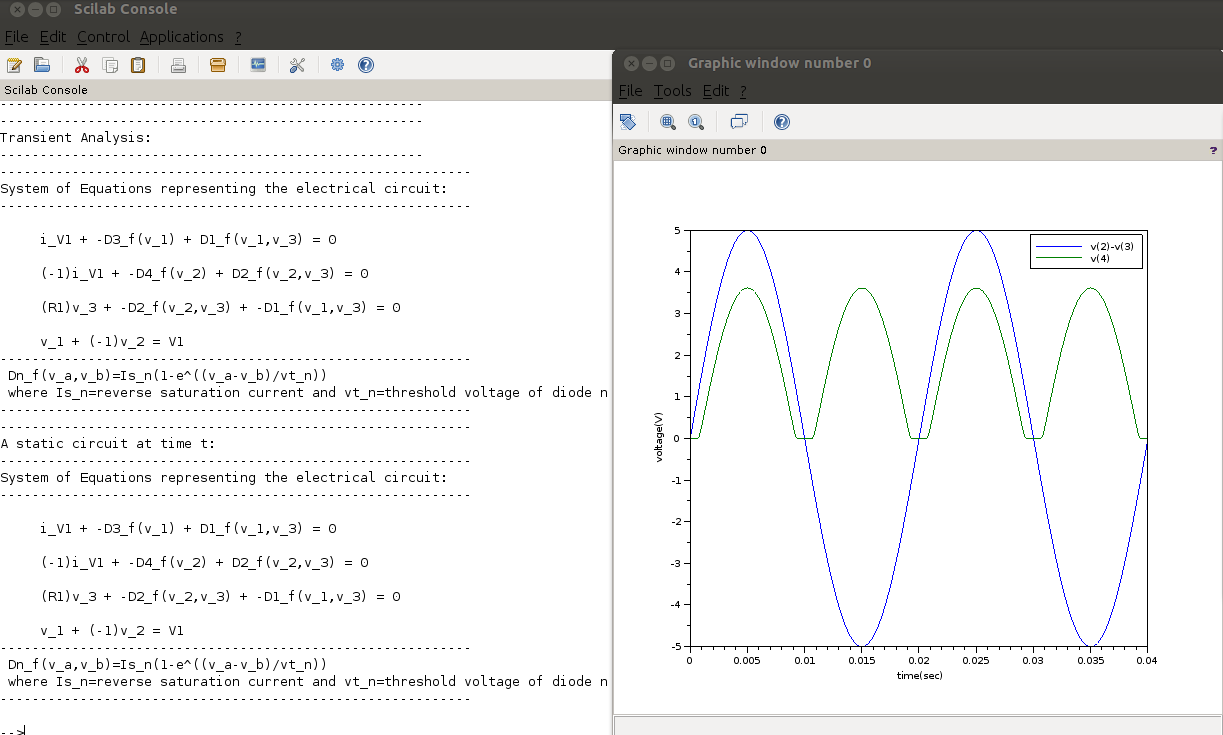
\includegraphics[width=1\linewidth]{figures/SMCSim-simulation.png}%If the fig is appearing too big/small, change the scaling factor 0.2
\caption{Scilab based simulation output}
\label{sci}
\end{center}
\end{figure}





